\documentclass{article}
%
%babel
\usepackage[romanian]{babel}
%
\usepackage{graphicx}
\usepackage{amsfonts}
\title{Proces adiabatic}
\author{Paliciuc Cosmin-Constantin\footnote{313AC}}
\date{}
\begin{document}
\maketitle
\begin{abstract}
Un proces adiabatic sau transformare adiabaticăeste o transformare a unui sistem termodinamic în care nu se produce un schimb de căldură cu exteriorul.
\end{abstract}
%
\section{Proces adiabatic}\label{intro}
Primul principiu al termodinamicii afirmă că energia este conservată. Pentru un sistem fizic macroscopic în repaus\cite{Bazil Popa} (variația energiei cinetice este zero), variația energiei interne a sistemului este egală cu energia schimbată cu mediul extern.Pentru o transformare elementară (adică care dă naștere unei mici variații a parametrilor care descriu sistemul). Prin urmare, un proces adiabatic este o transformare fără transfer de căldură, adică.
\section{Ecuația transformării adiabatice}
Transformarea adiabatică a gazului ideal poate fi descrisă de ecuația (1) unde p este presiunea, V este volumul, iar (doar pentru gaze perfecte):\( \gamma  =\frac{C_{p}}{C_{v}} =\frac{i+2}{i}\)\( C_{p}\) fiind capacitatea termică masică la presiune constantă, \( C_{V}\)  fiind capacitatea termică masică la volum constant, \( \gamma\) este exponentul adiabatic, iar \textit{i} reprezintă numărul gradelor de libertate ale gazului. \textit{i} poate fi 3 pentru gazele monoatomice, 5 pentru cele biatomice și 6 pentru celelalte gaze.\cite{Ioan Vlădea}
	\begin{equation}
	pV^{\gamma } = constant
	\end{equation}
	\begin{table}[htbp]
	\centering
	\caption{Unități de măsura}\label{tab:unit}
	\begin{tabular}{lll}
	\hline
	Nr.&Mărime&Valoare\\\hline
	1 &presiune&1 atm\\\hline
	2&volum&200l\\\hline
\end{tabular}
\end{table}
\newpage
\begin{figure}[ht]
\centering
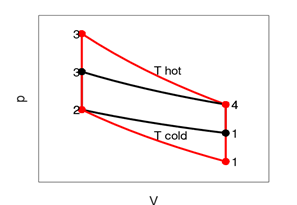
\includegraphics[scale=0.8]{Picture1.png}
\caption{Curba ce reprezintă variația presiunii în funcție de volum}\label{fig:figura}
\end{figure}
\section{Concluzii}
Transformarea adiabatică este un proces termodinamic în care sistemul termodinamic se schimbă dintr-o stare inițială într-o altă stare finală, fără a exista transfer de căldură între sistem și mediul extern. Acest lucru înseamnă că sistemul termodinamic nu primește nicio cantitate de căldură de la mediul extern și nici nu cedează căldură către mediul extern.
\begin{thebibliography}{a}
\bibitem{Bazil Popa}Bazil Popa (coord.), Manualul inginerului termotehnician, vol. 1, București: Editura Tehnică, 1986
\bibitem{Ioan Vlădea}Ioan Vlădea, Tratat de termodinamică tehnică și transmiterea căldurii, București: Editura Didactică și Pedagogică, 1974
\end{thebibliography}
\end{document}